\documentclass[fr,license=none]{../../../eplexercises}
\usepackage{multido}
\usepackage{float}
\usepackage{../../../eplcode}

% General info
\hypertitle[e ]{Systèmes informatiques 1}{3}{SINF}{1252}
{Brieuc Kaisin \and Cynthia Laureys}
{Olivier Bonaventure}
 
 
 % New colors
\definecolor{codegreen}{rgb}{0,0.6,0}
\definecolor{codegray}{rgb}{0.5,0.5,0.5}
\definecolor{backcolour}{rgb}{0.95,0.95,0.92}

\lstdefinestyle{mystyle}{
    backgroundcolor=\color{backcolour},   
    commentstyle=\color{codegreen},
    keywordstyle=\color{RedViolet},
    numberstyle=\tiny\color{codegray},
    stringstyle=\color{red},
    %basicstyle=\footnotesize,
    basicstyle=% change it if you want
        \ttfamily%
        \normalsize,
        %\lst@ifdisplaystyle\normalsize\fi,
    breakatwhitespace=false,         
    breaklines=true,                 
    captionpos=b,                    
    keepspaces=true,                 
    numbers=left,                    
    numbersep=5pt,                  
    showspaces=false,                
    showstringspaces=false,
    showtabs=false,                  
    tabsize=2,
    literate=%
    {é}{{\'e}}1
    {è}{{\`e}}1
    {à}{{\`a}}1
}


\lstset{style=mystyle, language=C}

%----------------------------------Macros--------------------------------------

\titleformat
{\section} % command
[display] % shape
{\bfseries\Large} % format
{\newpage Semaine \thesection} % label
{0.5ex} % sep
{} % before-code


\titleformat
{\subsection} % command
{\normalfont\large\bfseries} % format
{\thesubsection} % label
{0.5ex} % sep
{} % before-code

\newcommand\TODO{\textcolor{red}{TO DO}}
\newcommand\question[1]{\medskip\noindent\underline{\textbf{Question #1 :}}}
\newcommand\ingi[2]{\begin{center}\textbf{#1}\\ \url{#2}\end{center}}

\newcommand\qcm[2]
{
	\multido{\i=1+1}{#2}{
    \begin{figure}[H]
    	\centering
        \includegraphics[width=14cm]{#1/Q\i.PNG}
    \end{figure}}
}
%------------------------------------------------------------------------------   




%--------------------------------------S1--------------------------------------
\section{Introduction à Unix et au langage C} %1
\pagenumbering{arabic}
\subsection{QCM}
\qcm{QCMS1}{5}

\subsection{Exercices en bash}
\TODO

\subsection{Questions de base}
\question{1,2,6}
\begin{description}
\item[-Werror] Make all warnings into errors.
\item[-Wall] This enables all the warnings about constructions that some
users consider questionable, and that are easy to avoid (or modify to
prevent the warning), even in conjunction with macros. This also enables
some language-specific warnings described in C++ Dialect Options and
Objective-C and Objective-C++ Dialect Options.
\item[(-Wfatal-errors] This option causes the compiler to abort compilation
on
the first error occurred rather than trying to keep going and printing further
error messages.)
\end{description}

\question{3,7} Il faut rajouter \textit{return 0;} par exemple.

\question{8}\\
\url{http://sites.uclouvain.be/SystInfo/manpages/man3/atoi.3.html}\\
\url{http://sites.uclouvain.be/SystInfo/manpages/man3/strtol.3.html}

\question{9} EASY

\question{10} \TODO

\subsection{Petits programmes}

\question{1} \url{http://sites.uclouvain.be/SystInfo/manpages/man1/test.1.html}
\ingi{La commande test}{https://inginious.info.ucl.ac.be/course/LSINF1252/commandetest}
\begin{lstlisting}
#include <stdlib.h>
#include <stdio.h>
#include <string.h>

int eq(int n1, int n2)
{
	if(n1 == n2)
	return 0;
	else
	return 1;
}
int ge(int n1, int n2)
{
	if(n1 >= n2)
	return 0;
	else
	return 1;
}
int gt(int n1, int n2)
{
	if(n1 > n2)
	return 0;
	else
	return 1;
}
int le(int n1, int n2)
{
	if(n1 <= n2)
	return 0;
	else
	return 1;
}
int lt(int n1, int n2)
{
	if(n1 < n2)
	return 0;
	else
	return 1;
}
int ne(int n1, int n2)
{
	if(n1 != n2)
	return 0;
	else
	return 1;
}

int main(int argc, char *argv[])
{
	if(argc == 4)
	{
		int n1 = atoi(argv[1]);
		int n2 = atoi(argv[3]);
		
		if(strcmp(argv[2],"-eq") == 0)
			return eq(n1,n2);
		else if(strcmp(argv[2],"-ge") == 0)
			return ge(n1,n2);
		else if(strcmp(argv[2],"-gt") == 0)
			return gt(n1,n2);
		else if(strcmp(argv[2],"-le") == 0)
			return le(n1,n2);
		else if(strcmp(argv[2],"-lt") == 0)
			return lt(n1,n2);
		else if(strcmp(argv[2],"-ne") == 0)
			return ne(n1,n2);
		else
		printf("bad instruction ");
	}
	else
	{
		printf("Incorrect number of arguments (%d argument(s))\n",argc);
	}
	return 1;
}
\end{lstlisting}

\question{2} Fort semblable à la question 1.\\
\url{http://sites.uclouvain.be/SystInfo/manpages/man1/expr.1.html}

\question{3} \TODO

%--------------------------------------S2--------------------------------------
\section{Types de données} %2
\subsection{QCM}
\qcm{QCMS2}{13}

\subsection{Questions de base}
\question{1}
\begin{lstlisting}
#include <stdio.h>
#include <stdint.h>

int main(int argc, const char *argv[])
{
    printf("int : %d bytes\n", sizeof(int));
    printf("long : %d bytes\n", sizeof(long));
    printf("void* : %d bytes\n", sizeof(void *));
    printf("char* : %d bytes\n", sizeof(char *));
    printf("size_t : %d bytes\n", sizeof(size_t));
    printf("uint64_t : %d bytes\n", sizeof(uint64_t));
}
\end{lstlisting}

\question{2}
\begin{lstlisting}
void lsb(int number)
{
    int nbr = number;
    int bit = 32;
    while (nbr!=0)
    {
        nbr<<=1;
        bit--;
        //amelioration : effectuer bit-- avec des operations binaires
    }
    printf("Less significant bit of %d : %d", number, (int) pow(2,bit));
}
\end{lstlisting}

\question{3}
\begin{lstlisting}
#include <stdio.h>

int main()
{
    char* ptr = "Test";
    int i;
    for (i=0 ; i<4 ; i++){
        printf("%p\n", (void *) (ptr+i)); //or &ptr[i]
    }
}
\end{lstlisting}

\question{4}
\ingi{Echange de valeurs de fractions}{https://inginious.info.ucl.ac.be/course/LSINF1252/swap}
\begin{lstlisting}
void swap(struct fract_t *a, struct fract_t *b)
{
    int mem1 = a->num;
    int mem2 = a->denum;
    a->num = b->num;
    a->denum = b->denum;
    b->num = mem1;
    b->denum = mem2;
}
\end{lstlisting}

\question{5}
\begin{lstlisting}
#include <stdio.h>

int main()
{
    struct foo_t
    {
        char a;
        int b;
    };
    printf("Size of struct foo_t : %d bytes",sizeof(struct foo_t));
}
\end{lstlisting}

L'exécution de ce code affiche : \lstinline{Size of struct foo\_t : 8 bytes} et non 5 bytes (1+4) comme on pourrait le penser. Cela est dû à un phénomène d'alignement sur 32 bits du \textit{char a}.

\question{6}\\
\url{http://sites.uclouvain.be/SystInfo/manpages/man3/string.3.html}\\
\url{http://sites.uclouvain.be/SystInfo/manpages/man3/strlen.3.html}\\
\url{http://sites.uclouvain.be/SystInfo/manpages/man3/strcat.3.html}\\
\url{http://sites.uclouvain.be/SystInfo/manpages/man3/strcasecmp.3.html}\\
\textcolor{red}{Avertissement : ce code n'a pas encore été testé sur inginious (nombre d'essais limité)}

\ingi{Mini-projet : implémentation de strlen, strcat et strcasecmp}{https://inginious.info.ucl.ac.be/course/LSINF1252/mini-projet-string}
\begin{lstlisting}
size_t strlen(const char *str) {
    int i;
    for(i=0 ; str[i]!='\0';i++);
    return (size_t) i;
}

char *strcatt(char *destination, const char *source) {
    int i;
    int lenD = strlen(destination);
    int lenS = strlen(source);
    for (i=lenD ; i<lenD+lenS ; i++)
    {
        destination[i] = source[i-lenD];
    }
    destination[i+1] = '\0';
    return destination;
}

int strcasecmp(const char *s1, const char *s2) {
//TO DO
}
\end{lstlisting}

%--------------------------------------S3--------------------------------------
\section{Organisation de la mémoire} %3
\subsection{QCM}
\qcm{QCMS3}{7}

\subsection{Questions}

\question{1}
\begin{description}
\item[void *calloc(size\_t nmemb, size\_t size);] allocates memory for an array of
\textit{nmemb} elements of size bytes each and returns a pointer to the allocated
memory. The memory is set to zero. If \textit{nmemb} or size is 0, then
\textit{calloc()} returns either NULL, or a unique pointer value that can later be
successfully passed to \textit{free()}.
\item[void *malloc(size\_t size);] allocates \textit{size} bytes and returns a pointer
to the allocated memory. The memory is not cleared. If size is 0, then
\textit{malloc()} returns either NULL, or a unique pointer value that can later be
successfully passed to \textit{free()}.
\item[void free(void *ptr);] frees the memory space pointed to by \textit{ptr}, which
must have been returned by a previous call to \textit{malloc()}, \textit{calloc()} or
\textit{realloc()}. Otherwise, or if \textit{free(ptr)} has already been called
before, undefined behavior occurs. If ptr is NULL, no operation is performed.
\item[void *realloc(void *ptr, size\_t size);] changes the size of the memory block
pointed to by \textit{ptr} to \textit{size} bytes. The contents will be unchanged to
the minimum of the old and new sizes; newly allocated memory will be uninitialized. If
\textit{ptr} is NULL, then the call is equivalent to \textit{malloc(size)}, for all
values of \textit{size}; if \textit{size} is equal to zero, and \textit{ptr} is not
NULL, then the call is equivalent to \textit{free(ptr)}. Unless \textit{ptr} is NULL,
it must have been returned by an earlier call to \textit{malloc()}, \textit{calloc()}
or \textit{realloc()}. If the area pointed to was moved, a \textit{free(ptr)} is done.
\end{description}
\textit{calloc()} est plus lent que \textit{malloc()}.

\question{2} \TODO
\begin{lstlisting}
/**************************************
 * stack.c
 *
 * Programme d'exemple implementant un stack comme structure
 * chainee
 *
 **************************************/

#include <stdio.h>
#include <stdlib.h>

typedef struct fraction_t {
  int num;
  int den;
} fraction;

///AAA
typedef struct node_t
{
  struct fraction_t *data;
  struct node_t *next;
} node;

struct node_t *stack; // sommet de la pile

// ajoute un element au sommet de la pile
void push(struct fraction_t *f)
{
  struct node_t *n;
  n=(struct node_t *)malloc(sizeof(struct node_t));
  if(n==NULL)
    exit(EXIT_FAILURE);
  n->data = f;
  n->next = stack;
  stack = n;
}
// retire l'element au sommet de la pile
struct fraction_t * pop()
{
  if(stack==NULL)
    return NULL;
  // else
  struct fraction_t *r;
  struct node_t *removed=stack;
  r=stack->data;
  stack=stack->next;
  free(removed);
  return (r);
}

///BBB

// affiche le contenu de la pile
void display()
{
  struct node_t *t;
  t = stack;
  while(t!=NULL) {
    if(t->data!=NULL) {
      printf("Item at addr %p  :  Fraction %d/%d   Next %p\n",t,t->data->num,t->data->den,t->next);
    }
    else {
      printf("Bas du stack %p\n",t);
    }
    t=t->next;
  }
}

// exemple
int main(int argc, char *argv[]) {

  struct fraction_t demi={1,2};
  struct fraction_t tiers={1,3};
  struct fraction_t quart={1,4};
  struct fraction_t zero={0,1};

  // initialisation
  stack = (struct node_t *)malloc(sizeof(struct node_t));
  stack->next=NULL;
  stack->data=NULL;

  display();
  push(&zero);
  display(); %splay()
  push(&demi);
  push(&tiers);
  push(&quart);
  display();

  struct fraction_t *f=pop();
  if(f!=NULL)
    printf("Popped : %d/%d\n",f->num,f->den);

  return(EXIT_SUCCESS);
}
///CCC
\end{lstlisting}

\question{3}
\TODO

\question{4}
\TODO

\question{5}
\begin{lstlisting}
int main()
{
    int i;
    int a[3][3] = { {1,2,3} , {4,5,6} , {7,8,9} };
    int *b = &a;
    for(i=0 ; i<9 ; i++) printf("%d\n",*b+i);
    return 0;
}
\end{lstlisting}
Le programme affiche \textit{1,2,3,4,5,6,7,8,9}. Conclusion : le tableau \textit{a} est stocké ligne par ligne.

\question{6}
\begin{lstlisting}
int main()
{
    typedef struct
    {
        char c;
        long l;
        short s;
    } test_t;
    printf("Size of struct test_t : %d bytes",sizeof(test_t));
    return 0;
}
\end{lstlisting}
Le programme indique que la taille de la structure vaut 12 bytes.

\begin{lstlisting}
int main()
{
    typedef struct
    {
        char c;
        long l;
        short s;
    } test_t;
    test_t stru;
    stru.c = 4;
    stru.l = 456;
    stru.s = 42;
    int* ptrC = &stru.c;
    int* ptrL = &stru.l;
    int* ptrS = &stru.s;
    printf("%p, %p, %p",ptrC,ptrL,ptrS);
    return 0;
}
\end{lstlisting}
Le code ci-dessus affiche ceci : 0028FF14, 0028FF18, 0028FF1C.\\
Un moyen de réduire cette taille est d'écrire la structure ainsi :
\begin{lstlisting}
typedef struct
{
    char c;
    short s;
    long l;
} test_t;
\end{lstlisting}
Elle n'occupe maintenant plus que 8 bytes en mémoire.

\question{7}\\
\url{http://sites.uclouvain.be/SystInfo/manpages/man1/gcc.1.html}\\
\url{http://stackoverflow.com/questions/4306186/structure-padding-and-packing}
\begin{figure}[H]
\centering
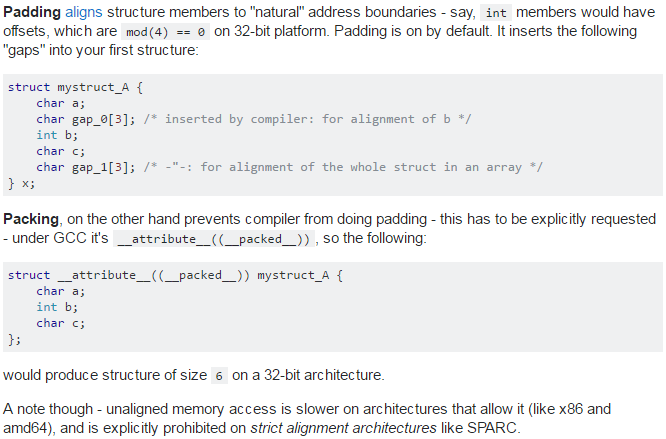
\includegraphics[width=14cm]{packed.PNG}
\end{figure}

\question{8}
\begin{lstlisting}
int global;
void main(void)
{
        int local;
        int *ptr1 = (int *)malloc(sizeof(*ptr1));
        int *ptr2 = (int *)malloc(sizeof(*ptr2));

        printf("global %p loc %p p1 %p p2 %p\n", &global, &local, ptr1, ptr2);
}
\end{lstlisting}
\TODO

\question{9}
\TODO

\question{10}
\ingi{Listes chaînées: concepts de base}{https://inginious.info.ucl.ac.be/course/LSINF1252/linked_lists_1}
\begin{lstlisting}
typedef struct node {
  int value;
  struct node *next;
} node;

size_t length(node *list)
{
    if(list==NULL)
        return 0;

    int count = 1;
    while (list->next != NULL)
    {
        list = list->next;
        count++;
    }

    return count;
}

size_t count(node *list, int value)
{
    if(list == NULL)
        return 0;

    int count = 0;
    while (list !=NULL)
    {
        if(list->value == value) count++;
        list = list->next;
    }
    return count;
}

int push(node **list, int value)
{
    node *n;
    n = (node *)malloc(sizeof(node));
    if(n == NULL)
        return -1;
    n->value = value;
    n->next = *list;
    *list = n;
    return 0;
}

int pop(node **list)
{
    if(list==NULL)
        return 0;

    int r;
    struct node *removed=*list;
    r = (*list)->value;
    *list = (*list)->next;
    free(removed);
    return r;
}

void free_list(node *list)
{
    struct node* tmp;

    while (list != NULL)
    {
        tmp = list;
        list = list->next;
        free(tmp);
    }
}
\end{lstlisting}

%--------------------------------------S4--------------------------------------
\section{Organisation des ordinateurs et étude de cas : IA32} %4
\subsection{QCM}
\TODO
\subsection{Exercices}

%--------------------------------------S5--------------------------------------
\section{Compléments de C et utilisation de plusieurs threads} %5
\subsection{QCM}
\TODO
\subsection{Exercices}

\question{1}
Souvent, nos threads vont vouloir retourner un pointeur vers une zone mémoire allouée
sur le tas. C'est pour ça que nos threads retournent \lstinline{void*}.

Du coup, \lstinline{pthread_join} doit recevoir un pointeur vers une variable du même
type que ce qu'on retourne, vu qu'elle va modifier la variable. Ce qu'on retourne
étant un \lstinline{void*}, l'argument de \lstinline{pthread_join} doit être un \lstinline{void**}.
\begin{itemize}
    \item \lstinline{void} ou tout autre type ne servirait à rien : \lstinline{pthread_join} ne
    pourrait pas modifier la moindre variable pour l'utilisateur.
    \item \lstinline{void*} ne permet que de retourner une valeur non-pointeur, et pas un pointeur
    (sauf en faisant un cast, ce qui est très dégueulasse). \lstinline{pthread_join} peut par
    exemple mettre un \lstinline{int}, mais pas un \lstinline{int*}
    \item \lstinline{void**} permet à \lstinline{pthread_join} de modifier l'argument et d'éventuellement y
    mettre un pointeur générique (\lstinline{void*})
\end{itemize}

\question{2}
\lstinline{pthread_create} doit modifier la structure qu'on lui passe en argument (il doit l'initialiser), tandis que \lstinline{pthread_join} se contente d'accéder aux valeurs qu'on lui passe en argument.

\question{3}
\TODO

\question{4}
\TODO

\question{5}
Environ $3000$ threads. En tout cas, c'est le maximum de ce qu'il est possible d'avoir sans qu'une segfault plutôt embêtante survient. On peut théoriquement en lancer $100000$ en réduisant la tâche qu'ils doivent accomplir, mais au bout d'un moment les threads lancés au début finissent par se terminer, libérant de la place pour les nouveaux. Toutes ces valeurs dépendent de l'ordinateur sur lequel les programmes sont utilisés.

\question{6}
\lstinline{pthread_exit} équivaut à un return dans une des fonctions de thread : ça arrête le thread courant.
\lstinline{exit} équivaut à un \lstinline{return} dans la fonction main : ça arrête le programme.

\question{7}
Lors de la fin de l'appel à \lstinline{launch} (qui s'exécute assez rapidement), le tableau \lstinline{v} alloué sur la pile n'est plus accessible et donc le programme foire (bon, c'est du garbage mais quand même).

\question{8}
De manière assez évidente, on n'atteint jamais $40000000$ mais des trucs intermédiaires. Il aurait fallu utiliser des mutex.

\question{9}
\TODO
%Implémenter un solveur de sudoku en utilisant un algorithme de remplissage aléatoire. Pas très intéressant, mais TODO


\subsection{Mini-projet : mesure de performance}

% //====================================================\\
% ||                         S6                         ||
% \\====================================================//
\section{Communication entre threads} %6
\subsection{QCM}
\TODO

\subsection{Exercices}

\question{1}
Les variables accessibles aux threads sont :
\begin{itemize}
    \item les variables globales;
    \item les variables dont un pointeur est l'argument d'un des threads;
    \item et les variables globales statiques si la fonction du thread est dans le même fichier (err, compilation unit) que cette variable.
\end{itemize}

La variables statique à une fonction n'est accessible que de cette fonction, mais sa valeur est "commune" à chaque thread, ce qui fait que ladite fonction n'est à priori pas thread-safe.

La variable locale est évidemment accessible qu'à partir de la fonction, et est réinitialisée à chaque appel de la fonction.

\question{2}
Plusieurs fois \lstinline|pthread_mutex_lock| : il se deadlock lui-même. Sauf si on a créé un mutex avec gestion des erreurs (\lstinline|PTHREAD_MUTEX_ERRORCHECK|) ; là il détecte le deadlock et renvoie une erreur.

Plusieurs fois \lstinline|pthread_mutex_unlock| : \emph{undefined behaviour} (en clair, ça crashe, ou alors ça délocke le mutex dans un autre thread)

\question{3}
Le premier marche (heureusement).

Le deuxième marche à priori quand même : on implémente presque le mécanisme interne de \lstinline{pthread_mutex_lock}.

\TODO vérifier

\question{4}
\TODO
% WHAT THE HELL IS GOING ON WITH HELGRIND ??????


% //====================================================\\
% ||                         S7                         ||
% \\====================================================//
\section{Les sémaphores} %7
\subsection{QCM}
\TODO
\subsection{Exercices}

\question{1}
Pour pouvoir modifier la structure : c'est une file d'attente (contenant les threads en attente) entre autre.

\question{2}
\begin{itemize}
    \item Le sémaphore est initialisé avec une valeur supérieure à la valeur maximale autorisée \lstinline|SEM_VALUE_MAX|.
    \item Le sémaphore a été initialisé pour être partagé entre plusieurs processus, mais l'OS ne supporte pas les sémaphores partagés entre processus.
\end{itemize}

\question{3}
Ce type d'attente est utile dans le cadre de systèmes temps réels. Dans certains cas, il peut arriver qu'une ressource à laquelle on veut accéder n'ait de sens que jusqu'à un certain moment, et qu'à partir d'un moment, ça ne serve plus rien d'attendre (typiquement, dans les réseaux, dans les gestions de fichiers, dans les systèmes embarqués ou temps réels). Dans ce cas, autant indiquer qu'on est près à attendre un certain temps, et passé ce temps ça ne sert plus à rien d'attendre.

Si le temps a été dépassé, la valeur de retour est de -1, et une erreur \lstinline|ETIMEDOUT| est présente. Si le sémaphore est bloqué au moment de l'appel, et que le temps d'attente est erroné, alors une erreur \lstinline|EINVAL| est présente.

\question{4}
Si lors de l'appel à \lstinline|sem_wait(&empty)|, il n'y a aucune case de libre, alors le thread va bloquer. Cela peut arriver parce qu'un producteur a rempli la dernière case juste avant, et qu'il est sorti de toutes ses sections critiques. Le problème, c'est que le seul autre thread qui peut incrémenter empty est un thread consommateur. Or, pour qu'un thread consommateur puisse s'exécuter, vider une case du buffer et incrémenter empty, il doit nécessairement s'approprier le mutex qui a été verrouillé par le producteur. De même, aucun consommateur n'était en train d'approvisionner le buffer (sinon il posséderait le mutex), et il est fort probable qu'aucun consommateur ne soit en train d'exécuter \lstinline|sem_post(&empty)|. On a donc une impossibilté pour le producteur de continuer : deadlock.

\question{5}
L'ordre dans lequel on libère les ressources importe peu : de toute façon, si un thread est bloqué sur les deux ressources, il devra attendre dans tous les cas l'autre avant de pouvoir s'exécuter. Et s'il attend sur une seule, c'est qu'il y a un bug.

Plus précisément, si une interruption a lieu avant \lstinline|sem_post(&empty)|, rien ne change. Si une interruption a lieu après \lstinline|pthread_mutex_unlock(&mutex)|, rien ne change non plus. Si une interruption a lieu entre les deux (le cas où une interruption survient entre les deux est implicitement géré par les fonctions appelées), alors on se retrouve avec l'indication d'une nouvelle case libre dans le buffer, mais avec un buffer toujours inaccessible. Si un thread était bloqué sur un \lstinline|sem_wait(&empty)|, il va peut-être être débloqué, mais il sera arrêté par son appel à \lstinline|pthread_mutex_lock(&mutex)| : le buffer n'a pas encore été libéré. Si aucun thread n'était bloqué sur \lstinline|sem_wait|, ils sont de toutes façons déjà bloqués sur le mutex. Donc, les autres threads doivent quand même attendre \lstinline|pthread_mutex_unlock| pour pouvoir enfin s'exécuter, et il n'y a donc pas plus de violation de section critique. Et comme ce sont deux appels non bloquant, aucun risque d'avoir un deadlock.

\question{6}
\TODO

% Ce qui suit est une spéculation de réponse ; j'avais l'impression que ça ne marchait pas, puis en écrivant je me suis rendu compte qu'il était bien probable que ça marche, et finalement j'ai vu que ça marchait.

%Supposons qu'il ne reste plus que deux threads avant que la barrière soit levée. Il est bien probable qu'une interruption ait lieu entre le \lstinline|pthread_mutex_unlock(&mutex)| et le moment où le \lstinline|if| et sa condition s'exécutent. Entre temps, vu que le mutex aura été changé, peut-être qu'un autre thread va venir modifier la valeur de \lstinline|count|, qu'il sortira lui aussi de sa section critique, et qu'il sera lui aussi interrompu avant le \lstinline|if|. Dans ce cas, si le premier thread revient à la charge, il verra que count vaut le nombre de thread requis, et va donc libérer les autres threads via sem_post, qui passeront ainsi le rendez-vous. Néanmoins, il restera un autre thread qui lui n'aura pas encore complètement fini. Mais il ne pourra faire qu'une seule chose : un sem_post supplémentaire, qui n'aura aucune influence sur le reste du déroulé du programme vu que tous les threads auront atteint la barrière quand cet espèce de foutoir aura lieu. En pratique, cette solution marche également, même si elle est moins clean que l'autre, et qu'elle peut faire plus de sem_post que nécessaire.

%TODO : je ne suis pas sûr, mais j'ai l'impression qu'en fait ça marche quand même


\question{7}
Avec $N$ threads, il y a exactement $N$ appels à \lstinline|sem_wait| qui décrémente la valeur du sémaphore, et $N+1$ appels à \lstinline|sem_post| qui incrémentent la valeur du sémaphore. Comme le sémaphore est initialisé à $0$ (pour que le premier thread arrivant soit déjà bloqué), à la sortie de la barrière, il aura la valeur $1$ ($0+(N+1)-N = 1$). Et normalement, tant qu'on implémente bien une égalité stricte, ça marche.

\question{8}
\TODO % Voir code.

\question{9}
Voir code fourni.

Etrangement, dans les cas où la section critique est relativement courte ($<60$), cela prend plus de temps d'utiliser des mutex que d'utiliser des sémaphores. Un peu contre-intuitif.

% //====================================================\\
% ||                         S8                         ||
% \\====================================================//
\section{Les processus} %8
\subsection{QCM}
\TODO
\subsection{Exercices}
\question{1}
La majorité des erreurs viennent de limitations mémoire :
\begin{itemize}
    \item pas assez de mémoire pour allouer les "necessary kernel structure" ;
    \item pas réussi à allouer assez de mémoire pour tout copier.
\end{itemize}

Un dernier cas est possible : on a atteint la limite supérieure au nombre total de processus pouvant être créés sur l'ordinateur (\#forkbomb).

Le plus simple pour provoquer une erreur est de créer un programme qui crée un nombre invraisemblable de processus, afin de saturer l'ordinateur. On peut par exemple utiliser le programme du QCM.

\question{2}
Généralement, c'est parce que la fonction a été mal appelée :
\begin{itemize}
    \item pas de processus avec cet identifiant, ou alors quelqu'un l'attend déjà ;
    \item mauvais arguments ;
    \item un signal a été reçu alors qu'on avait explicitement demandé à ne pas devoir en gérer.
\end{itemize}

\question{3}
Le processus père ne pourrait plus retrouver ses enfants.

\question{4}
On note $P$ le processus père, puis $A_1$ son fils de degré 1, $A_2$ le fild du fils, $B_1$ le second fild du père.
\begin{enumerate}
    \item Avant le premier fork : juste $P$
    \item Après le premier fork et avant le second fork : $P$ ainsi que $A_1$.
    \item Après le premier fork et avant le second fork : $P$ ainsi que $A_1$.
    \item Après le deuxième fork dans le processus fils : $A_1$ ainsi que $A_2$, et $P$ et ses enfants en arrière plan. Il ne va plus en créer, ses enfants non plus.
\end{enumerate}

On a donc 4 processus : $P$, $A_1$, $A_2$ et $B_1$.

\question{5}
% Flemme de faire autre chose que de l'ASCII art
\begin{lstlisting}
               Père P
                1252
               /     \
              /       \
       Fils A1        Fils B1
        1253       1255 ou 1254(*)
       /
      /
    Fils A2
1254 ou 1255(*)
\end{lstlisting}

(*) : ça dépend de si le père ou le fils s'exécute en premier après le premier appel à \lstinline|fork()|. Si le père commence (continue) avant le fils, B1 aura un pid de 1254 et A2 de 1255 ; si c'est le fils qui commence, $A_2$ aura le pid de 1254 et $B_1$ aura 1255.

\question{6}
Il va constituer une \emph{fork bomb} : des milliers de processus vont être créés, et ça va ralentir le système (vu qu'il doit, par principe, laisser chaque processus s'exécuter) et prendre beaucoup de ressources au niveau CPU et mémoire. Pour éviter ça, le kernel se protège des utilisateurs en instaurant une limite au nombre maximum de processus pouvant tourner en même temps sur un ordinateur. Si le maximum est atteint, plus aucun nouveau processus ne peut être créé. Par défaut, Linux ne copie pas immédiatement un processus et sa mémoire, mais ne copie que lorsqu'on modifie la mémoire (copy on write) ; du coup, ça ralentit les accidents mais c'est quand même dangereux.

\question{7}
Assez évidemment, le programme avec les processus prend bien plus de temps que le programme avec les threads.

\question{8}
\lstinline|ps()| indique qu'un processus est \og defunct \fg{} (il s'est terminé, et est un zombie). \lstinline|top| est plus explicite : il y a vraiment un zombie.

\question{9}
Note : \lstinline|system| est fortement déconseillé par le manuel lorsque le processus appelant a des privilèges au-dessus de la moyenne.

\TODO

\question{10}
\TODO

\question{11}
\TODO

\question{12}
Tous les processus descendent de \lstinline|systemd| (oh non... diront certains), et on voit bien tous les processus.

Petite subtilité : quand un processus est lancé deux fois, il n'apparait qu'une fois mais avec un petit 2 à côté. Autre subtilité : entre accolades ($\{ \}$), on a le nombre de threads enfants du processus.

\question{13}
Merci la documentation ;)

\question{14}
On voit bien le \emph{process id}, le \emph{parent process id} et le nombre de thread du processus père. On voit aussi qu'ils sont tous attachés au processus bash.

%--------------------------------------S9--------------------------------------
\section{Utilisation du système de fichiers et les \textit{pipe}} %9
\subsection{QCM}

\subsection{Exercices}

%--------------------------------------S10-------------------------------------
\section{Les signaux, les sémaphores nommés et le partage de fichiers} %10
\subsection{QCM}

\subsection{Exercices}

%--------------------------------------S11-------------------------------------
\section{La mémoire virtuelle et les fichiers mappés en mémoire} %11
\subsection{QCM}

\subsection{Exercices}

%--------------------------------------S12-------------------------------------
\section{Utilisations avancées de la mémoire virtuelle } %12
\subsection{QCM}

\subsection{Exercices}
\end{document}
